\documentclass[../main]{subfiles}

\input{chapter_header.tex}

\begin{document}

\chapter{GMU: Overview}

The Growth Monitoring Unit (GMU) is an intelligent subsystem integrated into the seed incubation plant to automate the observation of germination and early growth stages. It combines mechanical automation, image acquisition, and TinyML-based classification to continuously monitor the growth process with minimal human intervention.

\section{Objectives}
The Linear Rail Mechanism forms the core mechanical subsystem of the Growth Monitoring Unit (GMU). It provides precise, stable, and automated motion for the ESP32-CAM camera module to move across the seed trays in a controlled manner. The system is designed to achieve accurate image capture for plant growth monitoring and TinyML dataset generation.
\section{ESP32-Cam}
\begin{figure}[H] % H = exactly here
    \centering
    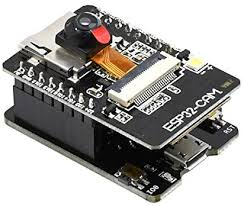
\includegraphics[width=0.3\textwidth]{pics/download.jpg} % replace with your image file
    \caption{ESP32-CAM module.}
    \label{fig:esp32cam}
\end{figure}
\paragraph{}
The ESP32-CAM is a compact, low-cost microcontroller board that combines the powerful ESP32 chip with a built-in camera module, making it ideal for IoT, computer vision, and smart imaging applications. It integrates a dual-core 32-bit processor, Wi-Fi, and Bluetooth connectivity, enabling wireless communication and real-time data processing. The module supports the OV2640 camera sensor, capable of capturing images at resolutions up to 1600x1200 pixels, and includes an onboard microSD card slot for local storage.
\paragraph{}
With programmable GPIO pins and support for various communication protocols (UART, SPI, I2C), the ESP32-CAM can interface with sensors, actuators, and external devices, providing a complete solution for embedded image processing and IoT development. Its small form factor and low power consumption make it suitable for portable, battery-powered, and edge-computing applications.


\section{System Overview}
The mechanism consists of two orthogonally arranged rails forming an X–Y stage:
\begin{itemize}
    \item The X-axis rail provides horizontal movement of the carriage across the seed tray.
    \item The Y-axis rail, mounted perpendicular to the X-axis, allows vertical or crosswise motion for additional positional control.
    \item Mounted on the Y-axis carriage is the ESP32-CAM module, which captures high-resolution images of the plants.
The movement of each axis is driven by stepper motors through timing belts or lead screws, ensuring high positional accuracy and repeatability.

\end{itemize}
\section{Hardware Components for Rail System}

\begin{table}[H]
    \centering
    %\caption{Hardware components used in GMU}
    \begin{tabularx} {\textwidth} {
            % >{\raggedright}p{3cm}
            % >{\raggedright}p{4cm}
            % >{\raggedright\arraybackslash}p{6cm}
            >{\raggedright}p{3.5cm}
            >{\raggedright}X
            >{\raggedright\arraybackslash}p{6cm}
        }
        \toprule
        \textbf{Component} & \textbf{Specification} & \textbf{Function} \\ \midrule
        Linear Rail & 300 mm Aluminum with MGN12H carriage & Enables smooth linear motion. \\
        Stepper Motor & NEMA 17 & Provides precise motion control. \\
        Pulley \& GT2 Belt & 6 mm width, 20T pulley & Converts rotary motion to linear displacement. \\
        Camera Module & ESP32-CAM & Captures seed tray images. \\
        Power Supply & 12V DC & Provides required operating voltage. \\
        Motor Driver & DRV8825 & Controls motor steps and direction. \\
        Limit Switch & Mechanical End-stop & Detects motion boundaries. \\
        Microcontroller & ESP32 & Controls motion, communication, and inference. \\
        \bottomrule
    \end{tabularx}
    \caption{Hardware components used in GMU}
\end{table}

\section{Working Principle}
%\begin{enumerate}
    %\item The ESP32 initializes motor control and camera modules.
    %\item The linear carriage moves across the tray, stopping at fixed points.
    %\item The ESP32-CAM captures images of seedlings.
    %\item The captured image is processed using an on-device TinyML model.
    %\item The classified growth stage and environmental data are transmitted to the central monitoring dashboard.
%\end{enumerate}
\vspace{3mm}
\resizebox{0.99\textwidth}{!}{
\begin{tikzpicture}[
    block/.style={
        rectangle, draw, thick, rounded corners,
        text width=5cm, align=center,
        minimum height=1.9cm, font=\Large, fill=white
    },
    smallblock/.style={
        rectangle, draw, thick, rounded corners,
        text width=4.8cm, align=center,
        minimum height=1.8cm, font=\large, fill=white
    },
    io/.style={
        trapezium, trapezium left angle=70, trapezium right angle=110,
        draw, thick, text width=5cm, align=center,
        minimum height=1.5cm, font=\Large, fill=white
    },
    arrow/.style={ultra thick,->,>=stealth},
    node distance=2cm and 2.8cm
]

% --- Main vertical flow ---
\node (start) [block,fill=green!10] {Start / System Initialization};
\node (esp) [block, below=of start,fill=green!10] {ESP32-CAM (Main Controller)};
\node (wifi) [block, below=of esp,fill=green!10] {Send Data via Wi-Fi to Flutter Dashboard};
\node (end) [io, below=of wifi,fill=green!10] {End of Scan Cycle / Output Data};

% --- Left branch (sensor side) ---
\node (limit) [smallblock, left=of esp, xshift=-2.8cm,fill=green!10] {Limit Switches (Home Detection)};
\node (image) [smallblock, below=of limit,fill=green!10] {Image Capture via ESP32-CAM};

% --- Right branch (motion + ML side) ---
\node (motor) [smallblock, right=of esp, xshift=2.8cm,fill=green!10] {Motor Driver + Stepper Motor (Linear Rail Movement)};
\node (tinyml) [smallblock, below=of motor,fill=green!10] {TinyML Processing Growth Stage Classification};

% --- Arrows: main vertical flow ---
\draw [arrow] (start) -- (esp);
\draw [arrow] (esp) -- (wifi);
\draw [arrow] (wifi) -- (end);

% --- Arrows: branches (curved outward to avoid crossing) ---
\draw [arrow] (esp) -- (limit);
\draw [arrow] (limit) -- (image);
\draw [arrow] (esp) -- (motor);
\draw [arrow] (motor) -- (tinyml);

% --- Arrows from branches to Wi-Fi ---
\draw [arrow] (image) -- (wifi.west);
\draw [arrow] (tinyml) -- (wifi.east);

\end{tikzpicture}
}

\vspace{0.8em}
%\textbf{Figure:} Workflow of the Growth Monitoring Unit (GMU) showing control, sensing, and data flow.
\vspace{3mm}


%\section{Mechanical Design}
The GMU frame is constructed using lightweight aluminum extrusion for stability. The camera carriage is mounted on a linear guide rail and driven by a timing belt connected to a stepper motor. End-stop switches prevent over-travel, ensuring system safety. The design ensures vibration-free image capture and precise camera positioning.

%\begin{figure}[H]
%\centering
%\includegraphics[width=0.85\textwidth]{gmu_blockdiagram.png}
%\caption{Block diagram of the Germination Monitoring Unit}
%\end{figure}

\section{Drive Mechanism and Camera Mount}
Motion in the linear rail is achieved through a belt-and-pulley drive system powered by NEMA 17 stepper motors and the camera carriage holds the ESP32-CAM module and moves along the linear rail.
\begin{itemize}
    \item Each motor drives a GT2 timing belt (6 mm width) with 20-tooth pulleys, converting rotary motion into precise linear displacement.

    \item The belts are tensioned using adjustable mounts to minimize backlash and vibration.

    \item The DRV8825 or A4988 motor driver provides current control, micro-stepping, and direction handling for smooth operation.
    he mount is 3D-printed or machined from acrylic or PLA material.

    \item It includes a tilt adjustment slot (±15°) for optimizing camera focus and angle.

     \item The camera mount is lightweight to reduce load on the motor and minimize vibration during image capture.

    \item Cable routing channels are designed along the carriage to organize power and data wires safely.
\end{itemize}

\vspace{0.5cm}
%\centering
\


%\centering
\resizebox{0.95\textwidth}{!}{
\begin{tikzpicture}[
    block/.style={
        rectangle, draw, thick, rounded corners,
        text width=4cm, align=center,
        minimum height=1.3cm, font=\large, fill=blue!10
    },
    arrow/.style={thick,->,>=stealth},
    node distance=1.5cm and 2.0cm
]

% --- Top: App communication ---
\node (app) [block, fill=green!10] {Wi-Fi / Flutter App Interface};

% --- Center: Main controller ---
\node (esp) [block, below=of app, fill=green!15] {ESP32-CAM \\ (Main Controller)};

% --- Bottom path: motion control ---
\node (driver) [block, below left=of esp, fill=green!15] {Motor Driver \\ (A4988 / DRV8825)};
\node (motor) [block, below=of driver, fill=green!15] {Stepper Motor \\ (NEMA 17)};
\node (rail) [block, below=of motor, fill=green!15] {Linear Rail + Belt + Carriage};

% --- Feedback path: limit switches ---
\node (limit) [block, below right=of esp, fill=green!15] {Limit Switches \\ (Home / End Detection)};

% --- Arrows ---
\draw [arrow, dashed] (app) -- (esp) node[midway,right]{Wi-Fi};
\draw [arrow] (esp) -- (driver);
\draw [arrow] (driver) -- (motor);
\draw [arrow] (motor) -- (rail);
\draw [arrow] (limit) -- (esp);

\end{tikzpicture}
}

%\vspace{0.1em}
{
\centering

%\textbf{Block diagram of drive mechanism of linear rail}

}
\vspace{0.5cm}

\section{Control and Communication}
Motor control signals (STEP and DIR) are generated by the ESP32. The A4988/DRV8825 driver regulates motor current and micro-stepping. The ESP32 communicates with the main incubator control system via Wi-Fi or LoRa. Image capture and processing are synchronized using internal timers.




\end{document}
